\documentclass{../source/Experiment}

\major{信息工程}
\name{}
\title{远程声控系统实现}
\stuid{}
\college{信息与电子工程学院}
\date{\today}
\lab{-}
\course{远程声控系统实现}
\instructor{张朝阳}
\grades{}
\expname{}
\exptype{}
\partner{}
\begin{document}
\makecover

\section{问题背景}
实现一个远程声音控制系统。首先采集不同的语音指示信号,进行适当压缩;然后通过噪声信道实现远程传输,远端接收后再通过适当计算识别出是何指示,最后送入一个处于未知状态、但能控/能观的控制系统,完成不同的控制动作

\section{问题分析}
分析此问题,可以分为信号采集、信号传输、语音识别、指令控制四部分。

具体流程图如下:
\begin{figure}[H]
    \centering
    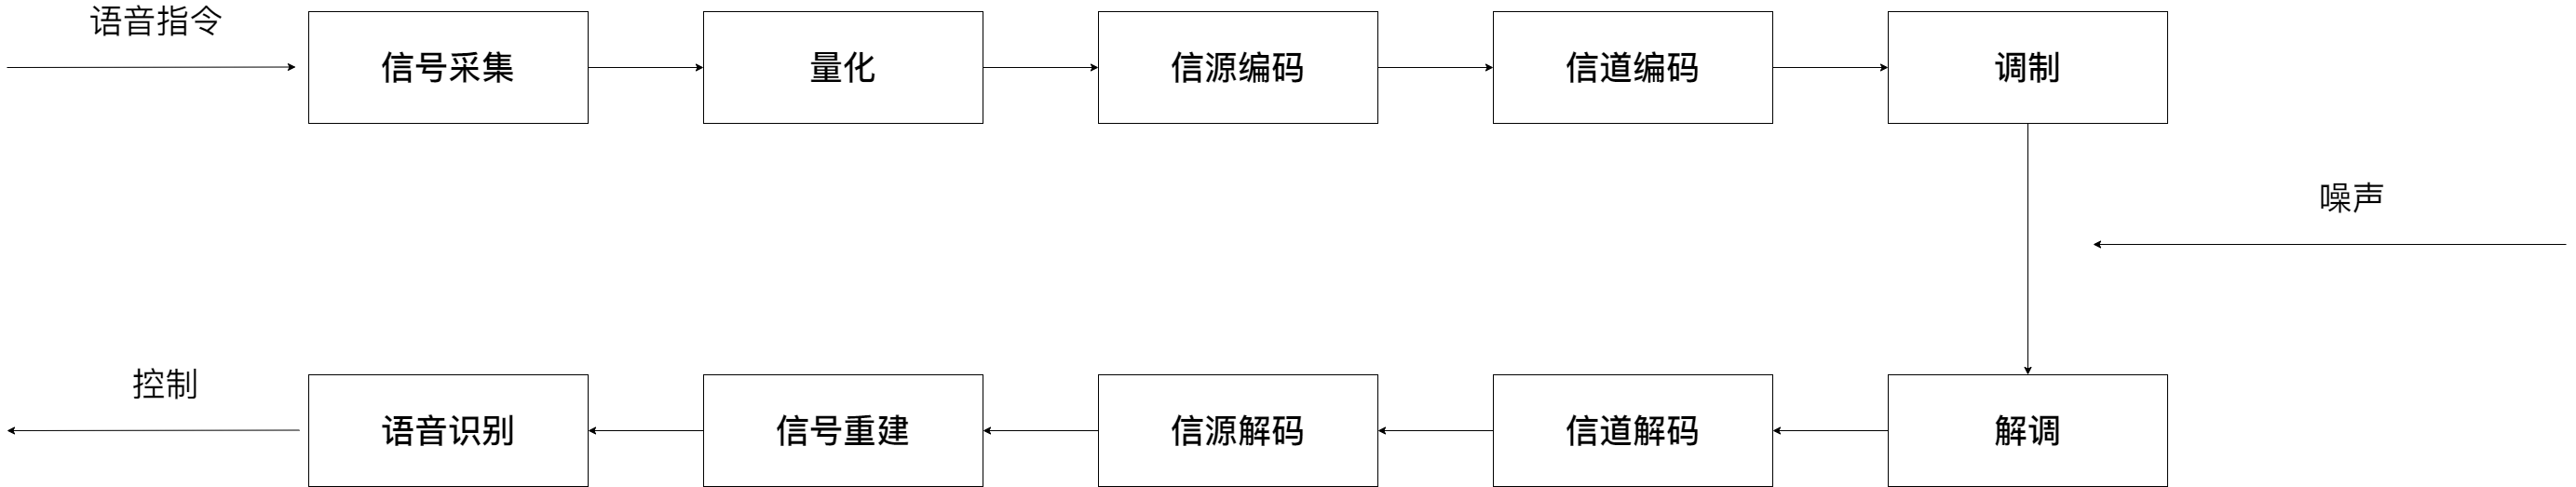
\includegraphics[width = 1\textwidth]{流程图}
    \caption{流程图}
\end{figure}
其中信号采集可以直接使用matlab自带的函数实现。

信号传输包括了信号量化、信源编码、信道编码、调制解调、信道译码、信源译码六个过程。其中信源编码我们采用了霍夫曼编码,信道编码采用了卷积码,调制选用了BPSK调制,并人为引入了高斯白噪声模拟传输时的噪声。

语音识别部分通过Matlab的已经训练好的模型进行识别。

\section{具体实现过程}
\subsection{语音指令信号采集}
由于人发出的信号被麦克风采集到时,是连续的模拟信号,所以需要将其转换为数字信号,才能被我们后续的处理。

这里我们直接采用了Matlab中的audiorecorder函数进行了录制,设置采用率为16000Hz,采样位数16bits,通道数1,录音时长1s。此处我们录制右转指令“right”,得到时域图和频域图如下:

\begin{figure}[H]
    \centering
    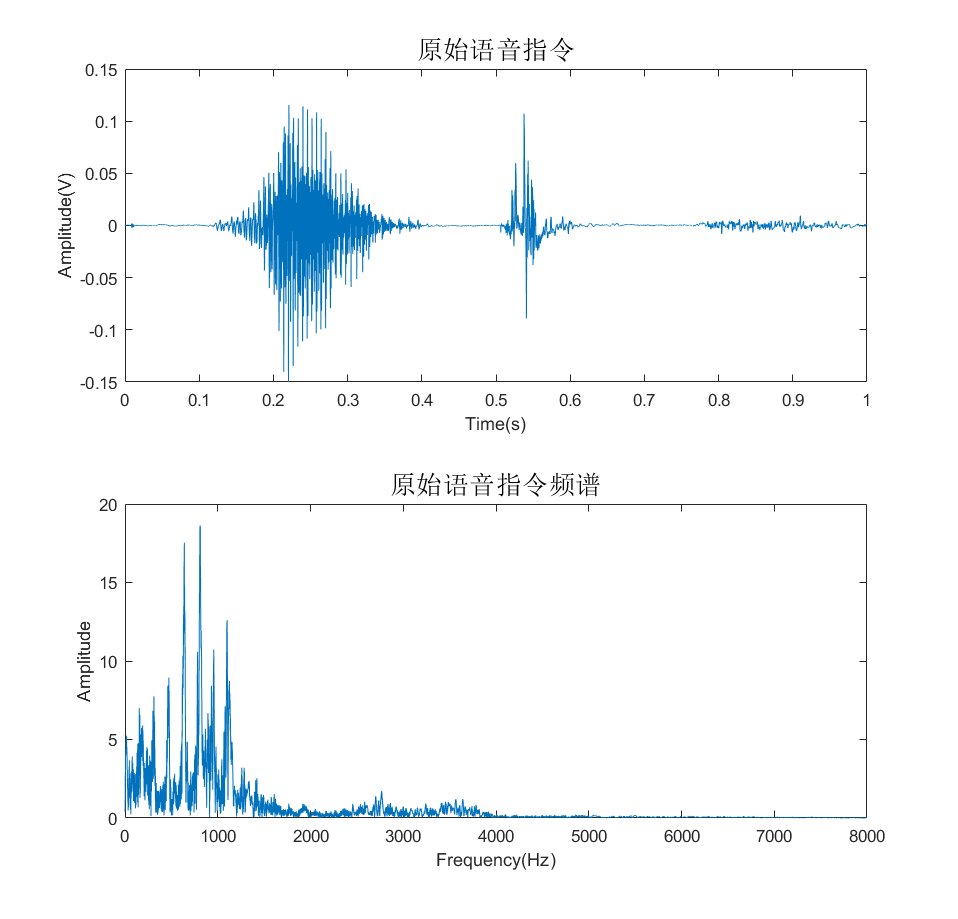
\includegraphics[width = 0.9\textwidth]{MyAudio}
    \caption{采集到的语音指令信号时域和频域图}
\end{figure}

\subsection{信号量化}
采样到的电压幅度值是模拟的,为了后续的处理,我们还需要对其进行量化编码,使其电压幅度值映射到离散电平,并用二进制表示。此处我们使用了量化等级为8的量化器进行量化,具体分辨率为为
$$
    q = \frac{V_{max} - V_{min}}{2^N} = \frac{1- (-1)}{2^8} = 3.90625\times 10^{-3}V
$$

\subsection{信源编码}
信源编码又称为数据压缩,是一种以提高通信有效性为目的而对信源符号进行的变换,或者说为了减少或消除信源冗余度而进行的信源符号变换。

而观察我们的信号频域图可以发现,信号在不同的频率处高度并不一样,而且差异很大,所以我们选择了我们所学过的不等长编码中的霍夫曼编码,用以压缩信号和节省带宽。

实验中我们先计算各个负号出现的概率,再利用Matlab自带的函数huffmandict生成字典,在通过huffmanenco 生成霍夫曼编码。

以下为编码结果:
\begin{lstlisting}[language = matlab]
            ----- Source Encode -----
            平均码长 : 2.181875
            信源熵 : 2.102782
            编码效率 : 0.475560
            编码前字符串总长度 : 128000
            编码后字符串二进制总长度 : 34910
            压缩率 : 3.666571
            \end{lstlisting}

\subsection{信道编码}
实际信号传输的过程中,信道存在噪声和干扰,会使得我们接受的码字和发送的码字之间存在错误。所以可以通过信道编码,在发送的信息码元中加入一些冗余码元,进行监督,从而能够在出错时进行纠正,达到改善传输和纠错的目的。

由于课程中并没有讲信道编码,所以在查阅资料后,我采用了卷积码对信道进行编码。

卷积编码属于信道编码的一种,信道编码的作用是通过增加冗余来提高传输的准确性,当然这样会导致信息传输速率的下降。卷积码是一种前向纠错码,比一般的分组码可以拥有更好的性能,因为卷积编码输出的每个码即和当前输入数据有关,也和之前输入的数据有关。

一般用(n,k,L)来描述卷积码,即我们输入k个信息比特经过卷积码编成n个比特(n一定是大于k的,就是加进去了冗余来进行纠错),L是编码的约束长度。编码器由n个模2加法器和L*k-1级移位寄存器组成。

此处我们采用了(2,1,7)卷积编辑器进行编码,而Matlab中有内置的卷积吗实现的函数即:


\begin{lstlisting}[language = matlab]
            trellis = poly2trellis(ConstraintLength,CodeGenerator);
            code_data = convenc(P_data,trellis);
            \end{lstlisting}

其中poly2trellis函数将 (2,1,7) 卷积码生成了 Matlab 的网格表达式,随后利用convenc函数对输入序列进行了编码。

编码结果如下:
\begin{lstlisting}[language = matlab]
            ----- Channel Encode -----
            信道编码前字符串长度 : 34910
            信道编码后字符串长度 : 69820
            编码速率:0.5
            \end{lstlisting}

\subsection{调制解调}
由于课程中并没有讲调制和解调,所以在查阅资料后,我采用了相移键控进行调制。此处我们采用二进制相移键控BPSK,并且为了模拟实际传输过程中的噪声干扰,我们在调制好的信号中加入了加性高斯白噪声,取信噪比为10dB。

此处用Matlab中的函数
\begin{lstlisting}[language = matlab]
            bpsk_out = pskmod(channel_encode,2);
            \end{lstlisting}
进行BPSK调制
\begin{lstlisting}[language = matlab]
            awgn_out = awgn(bpsk_out, 10);
            \end{lstlisting}
进行高斯噪声的加入。

而解调时任然使用pskmod函数。

结果如下:

\begin{lstlisting}[language = matlab]
            -------- Modulation --------
            调制解调出错数 : 0
            调制解调误码率 : 0.000000
            \end{lstlisting}

\subsection{信道译码}
信道编码采用的是卷积码,译码时使用vitdec函数进行译码。

结果如下:
\begin{lstlisting}[language = matlab]
            -------- Channel Decode --------
            信道解码出错数 : 0
            信道解码误码率 : 0.000000
            \end{lstlisting}


\subsection{信源译码}
信源编码采用的是霍夫曼编码,译码采用huffmandeco函数。

结果如下:
\begin{lstlisting}[language = matlab]
            -------- Channel Decode --------
            信道解码出错数 : 0
            信道解码误码率 : 0.000000
            \end{lstlisting}

\section{信号重建}
信号重建只需要将信源译码得到的离散信号和量化分辨率相乘再减一。
\begin{figure}[H]
    \centering
    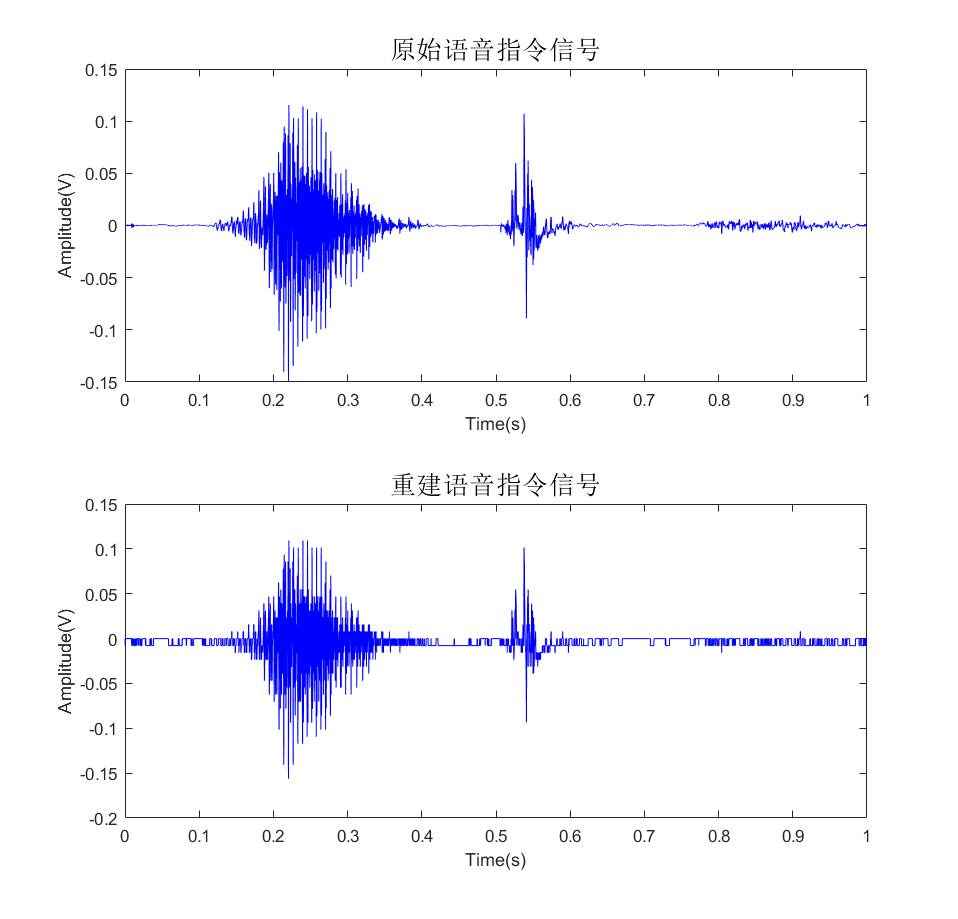
\includegraphics[width = 0.9\textwidth]{Compare}
    \caption{原始信号和重建信号时域对比}
\end{figure}

\begin{figure}
    \centering
    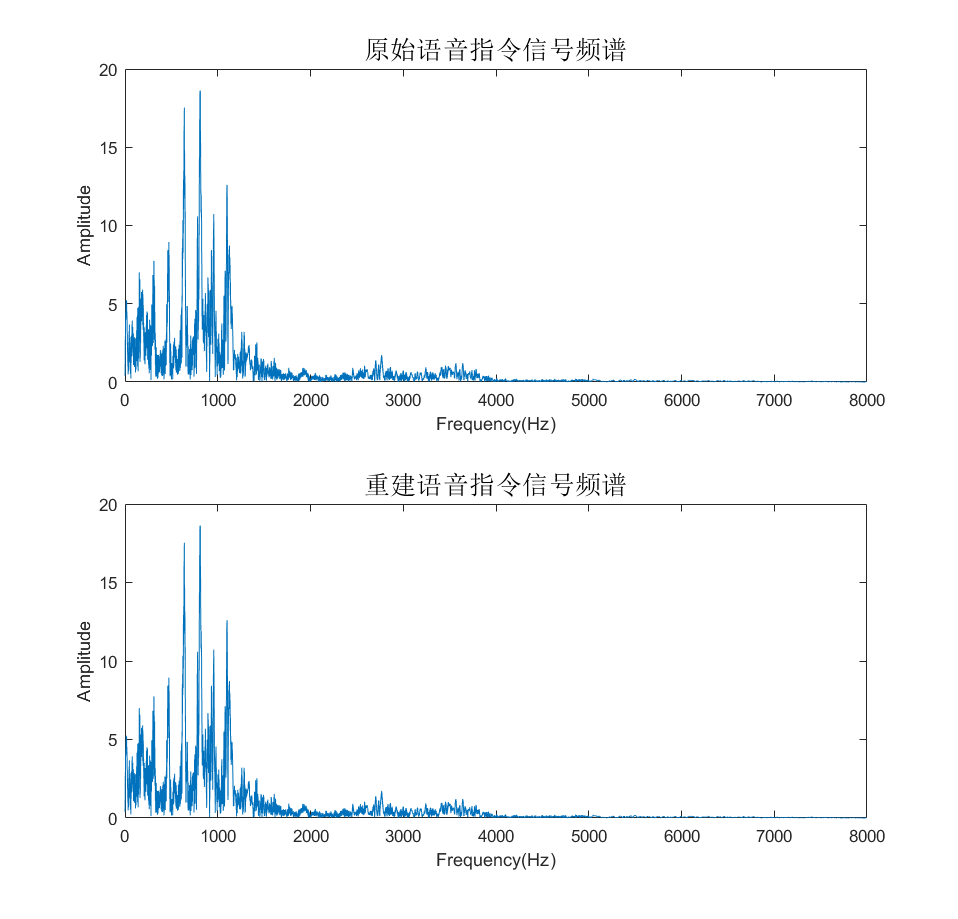
\includegraphics[width = 0.9\textwidth]{Compare2}
    \caption{原始信号和重建信号频域对比}
\end{figure}

此外我们使用了Matlab中的mse函数计算了原始信号和重建信号的均方误差。结果如下:
\begin{lstlisting}[language = matlab]
            -------- Mean Square Erro --------
            均方误差: 0.000022
            \end{lstlisting}

可以看出,无论是通过信号时域和频域对比图还是通过均方误差来看,原始信号和重建信号的差异都非常小。
\subsection{语音识别}
语音识别部分,通过查阅资料学习,我们采用了现在普遍采用的CNN模型进行处理,此处我们直接使用了Matlab 的 Deep Learning Toolbox中预先训练好的模型。改模型可以识别简单的go,stop,yes,no,up down,left,right,on,off十条指令。并且本次实验我们以指令“right”为例。最后识别结果如下:
\begin{lstlisting}[language = matlab]
            -------- Speech Recognition --------
            识别结果:right
            \end{lstlisting}

\subsection{控制}
控制阶段,我们假设了一个有限状态机进行动作的控制,状态机根据输入的指令以及当前的状态共同决定下一个状态。从而进行控制。

\section{心得体会}
刚开始本次试验时,我觉得十分棘手,虽然课程中已经讲了许多的相关知识,但是自己缺乏对整个信号传输以及控制的系统性认知,所以导致刚开始时无从下手。

在此基础上,我向同学以及学长请教,首先大概理清了整个问题大概的实现过程。之后,我开始着手一步步对,每一个过程进行分析,期间除了回顾学过的信源编码等已经上过的知识,也查阅学习了如信道编码和调制解调等许多新知识。

同时也查阅了相关实验的文章、博客教程,最后通过Matlab对该问题进行了简单的实现。

\section{参考文献}

1. matlab有关卷积码编译码的函数.https://blog.csdn.net/xiangziling/article/details/106908643

2. matlab实现卷积编码'适合小白理解学习'.https://blog.csdn.net/wang6350339/article/details/94837370

3. PSK原理及MATLAB仿真.https://www.docin.com/p-680830415.html

4. Pskmod函数\_Matlab笔记——AWGN函数详解与实例——AWGN加性高斯白噪声+QPSK调制.https://blog.csdn.net/weixin\_39585675/article/details/113312105

5. 薛年喜.MATLAB 在数字信号处理中的应用 [M]. 北京: 清华大学出版社,2003.

6. 郑君里, 应启绗, 杨为理. 信号与系统 [M]. 北京: 高等教育出版社,2000

\section{附录:实验代码}
\lstinputlisting[
    language       =   Matlab,
    title     =   {实验代码}
]{大作业/main.m}



\end{document}